\section{Experimental Evaluation: comparing provenances}
\label{sec:experiments}

\begin{figure}[t]
  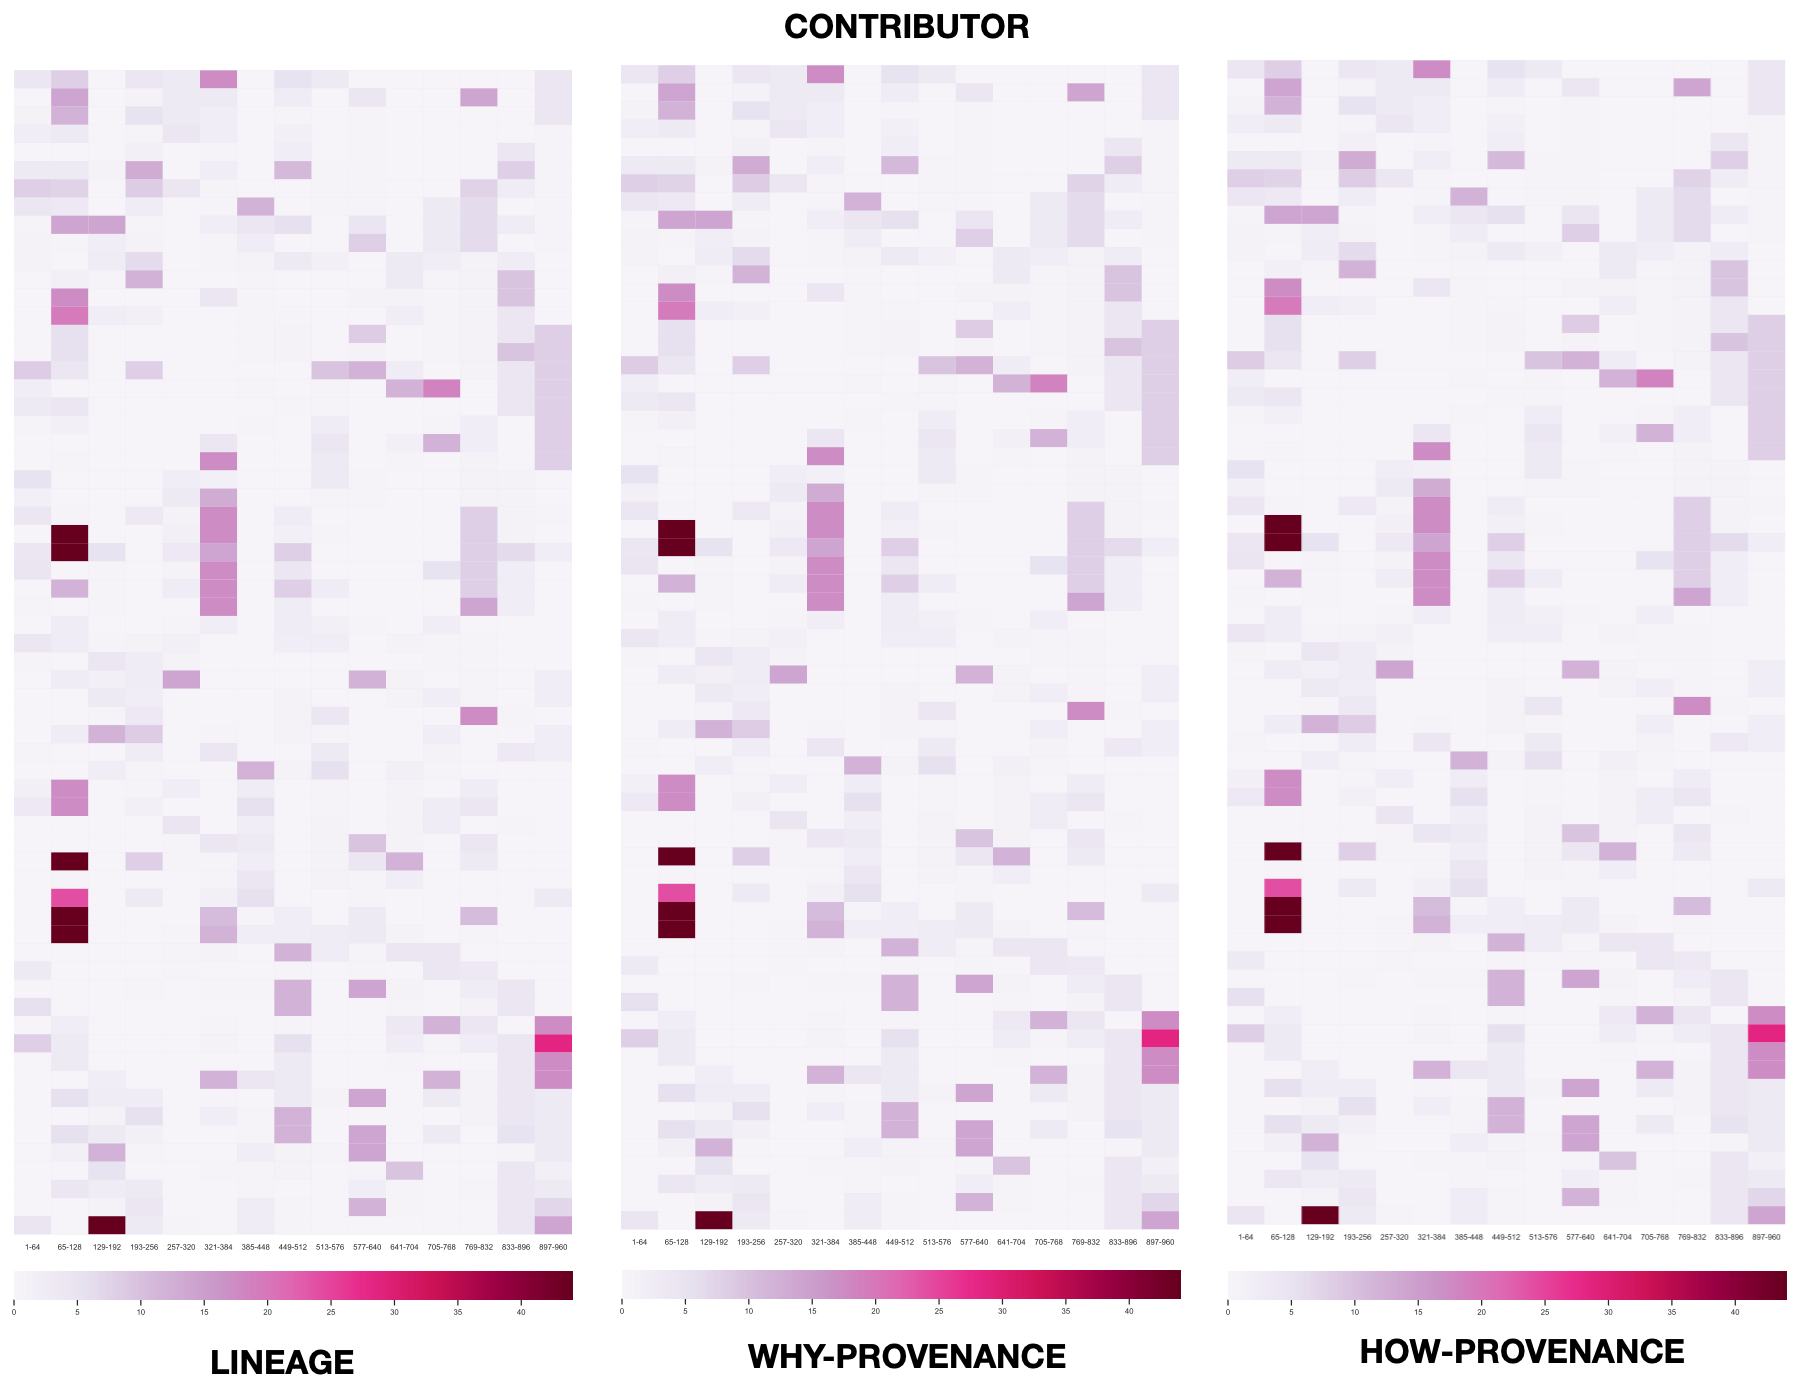
\includegraphics[width=1\textwidth]{figures/paper_based_comparison}
  \caption{Comparison of three DS on the same table \texttt{contributor} using the distribution given by the queries retrieved from papers.}
  \label{figure:comparison_on_papers}
\end{figure}

In this paper, we perform our experiments on GtoPdband in particular we focus on target families, all of those are described in webpages. 
GtoPdb in particular identifies eight family types: \emph{GPCR}, \emph{Ion channels}, \emph{NHRs}, \emph{Kinases}, \emph{Catalytic receptors}, \emph{Transporters}, \emph{Enzymes} and \emph{Other protein targets}.  

When a paper uses data from GtoPdb, it can cite the full database, the family webpage of interest, or a subset of data extracted with a query. 
In this work we consider a full-fledged data citation context in which papers cite the specific \emph{data} subset of interest and not the webpage or the full database acting as data proxies.  
Therefore, when a paper cites family data, it is actually citing a set of queries needed to retrieve all the information provided by the family webpage, i.e. one query for each section composing a page, as depicted in Figure \ref{figure:family_structure}. 
The figure maps the structure of one family, ``Adenosine receptors'', and the queries to obtain the information to build the corresponding page, apart from the list of references. 
In GtoPdb, all family pages share a similar structure (the only differences may be the presence/absence and length of the receptors lists, further readings, and contributors sections).
The same queries are therefore used to build all other pages by simply changing the family id (which, in our example, is 3). All these queries are SPJ. 

As already stated, many papers that draw information from the GtoPdb website\footnote{\url{https://www.guidetopharmacology.org}} cite papers published every two years by the GtoPdb Committee on Receptor Nomenclature and Drug Classification (NC-IUPHAR).
To obtain a set of citations capable of representing what actually happens, we consider a paper subset citing the 2018 GtoPdb~\citep{iuphar2018} data paper. 
At the time of writing, this paper received more than $1200$ citations. 

As explained in Section \ref{section:use_case}, in the papers published in the British Journal of Clinical Pharmacology, that cite GtoPdb, the name of families are hyperlinks that point to the corresponding webpages.
We considered all the $460$ papers in BJCP citing \citep{iuphar2018} as of February 2020. 
URL references to family pages were automatically extracted to guide in building the queries to produce corresponding webpages.
A total of $5,945$ different queries were built in this way. \footnote{For reproducibility purposes, the code we used for our experiments and all the produced queries can be found at the following link: \url{https://bitbucket.org/dennis_dosso/credit_distribution_project}.}

Figure \ref{figure:comparison_on_papers} shows the heat-maps obtained by three different DS on the table \texttt{contributor}.
It is immediately evident that the result of the distribution is the same with the three strategies. The same result is also obtained in the other tables of the database used by the considered queries. 
Why is that? 
It is the case that the conditions in which we produced this experiment are quite peculiar. The queries that we used all share similar characteristics. They are all SPJ queries, each of them utilizes each table only once in the join condition (there are no self-joins) and all the joins are made using key attributes. 
In this particular condition, each tuple of the output presents: (i) a how-provenance that is a single monomial with coefficient $1$ and exponent $1$ in each variable; (ii) a why-provenance that is composed by only one witness; (iii) a lineage that coincides with the only witness in the witness basis.
It is easy to see how, given these queries, the three distributions act in the same way.
The credit is always uniformly distributed among the tuples appearing in each provenance. 

To better clarify what is happening, let us consider one of the types of queries used to build the output webpage, as shown in Figure \ref{figure:family_structure}:
\begin{verbatim}
	Q3: SELECT c.first_names, c.surname
	FROM contributor2family AS cf JOIN contributor AS c ON 
	cf.contributor_id = c.contributor_id 
	WHERE f.family_id = 3
\end{verbatim}

\texttt{Q3} returns a series of $10$ tuples from the version of GtoPdb we considered. 
The first tuple produced by this query, \texttt{<Bertil B., Fredholm>}, has $c_{939} \cdot c2f_{496}$ as provenance polynomial.
$c_{939}$ represents the provenance token of a tuple in \texttt{contributor}, the same for $c2f_{496}$ in table \texttt{contributor2family}. 
It is easy to see that the why-provenance of this tuple is $\{\{c_{939}, cf_{496} \}\}$ and its lineage is $\{c_{939}, c2f_{496} \}$.
Therefore, the credit assigned to these tuples is $1/2$ using all three DS.
This actually happens for each tuple of the output of each query of GtoPdb, thus making the distributions equivalent.

This is not always the case with general queries and other databases. As we showed in the examples in the previous section, when two or more tuples are merged by the effect of a projection or union, alternatives appear. These are represented as multiple witnesses and multiple monomials. 

To give an example of how the CDS can differ from one another in their behavior, let us consider a different query:
\begin{verbatim}
	Q4: SELECT f.name AS name
	FROM family AS F JOIN
	(SELECT DISTINCT f.family_id, f.name
	FROM "family" AS f JOIN contributor2family AS cf ON 
	f.family_id = cf.family_id 
	JOIN contributor c ON 
	cf.contributor_id = c.contributor_id 
	WHERE c.country = 'UK') AS R 
	ON F.name = R.name
\end{verbatim}

Here the innermost query retrieves all the names and ids of the families written by an author from the UK producing a relation called $R$. This relation is then joined with the table \texttt{family} on the attribute \texttt{name}. 

One output tuple of this query is \texttt{<Histamine receptors>}, that has the following provenance polynomial:
\[
\begin{array}{c}
	f_{625}(f_{625} c2f_{656} c_{184} + f_{625} c2f_{113} c_{180} + f_{625} c2f_{283} c_{198} +\\ 
	+ f_{625} c2f_{550} c_{865} + f_{625} c2f_{573} c_{101} + f_{625} c2f_{95} c_{109} )
\end{array}
\]

As already discussed, the different monomials represent possible \emph{alternatives} of combinations of tuples that produce the considered output tuple. 
Tuple $f_{625}$ is used each time with different joins, thus it appears in each monomial. 
The last join, performed in the outmost query, is responsible for the final multiplication of $f_{625}$ with the rest of the polynomial between parenthesis.

From this polynomial we compute the why-provenance as a set of six different witnesses:
\[
\begin{array}{c}
\{\{ f_{625}, c2f_{656}, c_{184} \}, \\ \{ f_{625}, c2f_{113}, c_{180} \} \\
\{ f_{625}, c2f_{283}, c_{198} \}, \\ \{ f_{625}, c2f_{550}, c_{865} \},\\
 \{ f_{625}, c2f_{573}, c_{101}\} , \\ \{f_{625}, c2f_{95}, c_{109} \}\}	\\
\end{array}
\]

And corresponding lineage:
\[
\begin{array}{c}
	\{ f_{625}, c2f_{656}, c_{184}, c2f_{113}, c_{180}, 
  c2f_{283}, c_{198}, c2f_{550}, c_{865}, 
  c2f_{573}, c_{101}, c2f_{95}, c_{109}\}
\end{array}
\]

\begin{figure}[tb]
  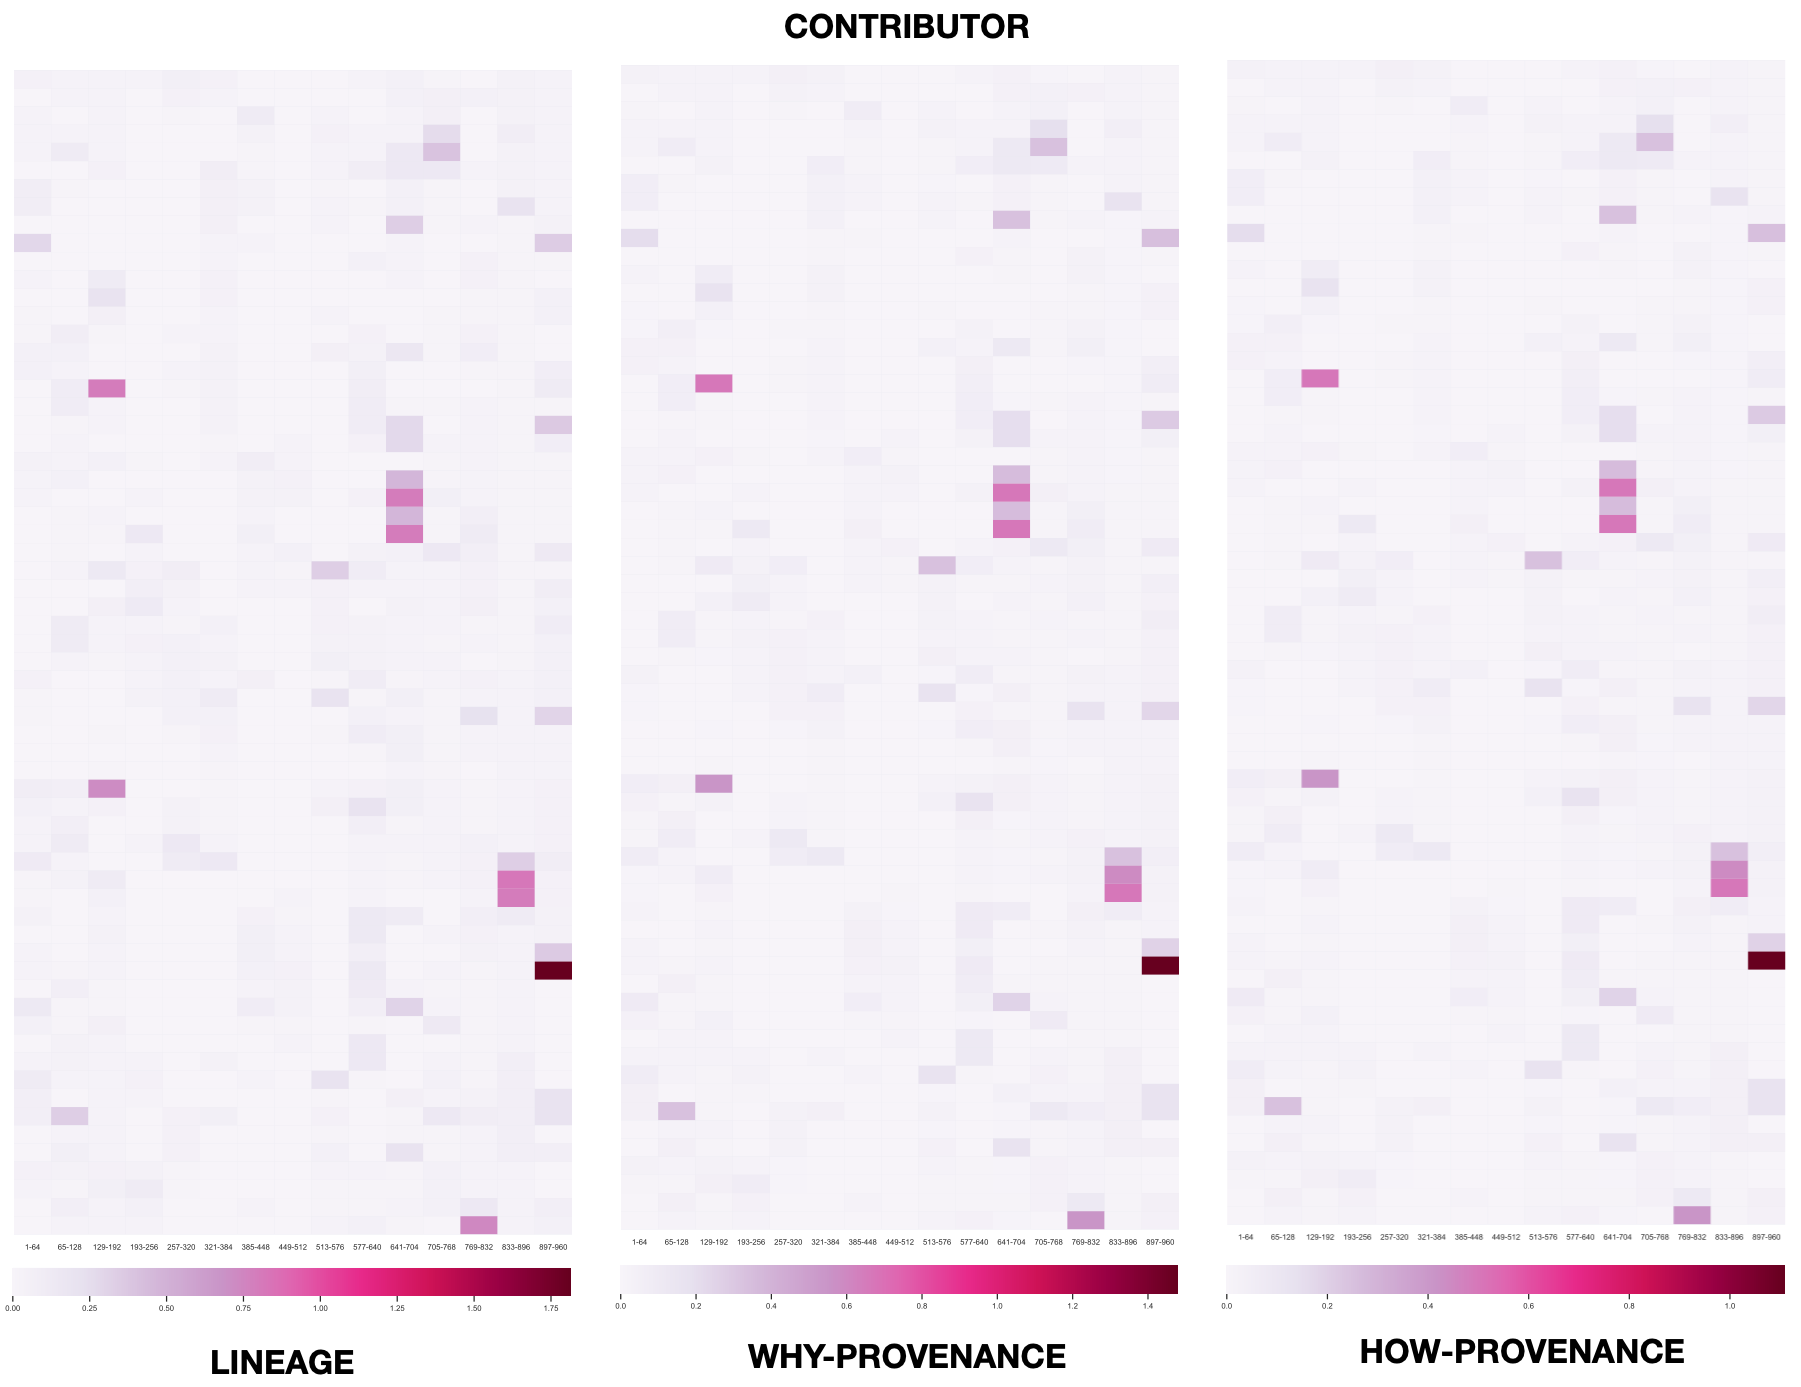
\includegraphics[width=1\textwidth]{figures/synthetic_queries}
  \caption{Comparison of three DS on the same table \texttt{family} after the distribution of the credit connected to query \texttt{Q4}.}
  \label{figure:comparison_on_synthetic_query_1}
\end{figure}

This was only one tuple among the $86$ obtained from this query. If we assign credit $1$ to all these tuples and distribute it with the different strategies, we obtain the result shown in Figure \ref{figure:comparison_on_synthetic_query_1} for the table \texttt{contributor}.
At first sight, it may appear that the three distributions produce the same result. This is only partially true: the heat maps appear equal, but the absolute values assigned to each tuple are different. 
This is more evident if we look at the legend of each heat-map, where the maximum quantity of credit is different for each distribution. The one performed through lineage is around $1.8$, the why-provenance's one is around $1.4$, and the one based on how-provenance is around $1.1$. 

To understand what is happening with this query in this specific table, consider the output tuple \texttt{<Histamine receptors>} and its provenances, as discussed above.
Let us focus on its lineage. There are a total of six authors for this family and $13$ tuples in total in the lineage. 
Thus, using the lineage-based DS, each tuple belonging to the \texttt{contributor} table (i.e. $c_{184}, c_{180}, c_{198}, c_{865}, c_{101}, c_{109}$) receives credit equal to $1/13$.
Tuple $f_{625}$ too receives a portion of credit equal to $1/13$.

Let us consider now why-provenance. Tuple $f_{625}$ appears six times in six different witnesses composed of $3$ elements each. From each witness it receives a portion of credit equal to $1/18$, thus its total credit is $1/3$.
On the other hand, all the authors appear only once in each witness, thus each of them receives credit $1/18$. 
In this case, why-provenance is recognizing more credit to tuple $f_{625}$, since it appears in each witness. The consequence is that this distribution is equally \emph{subtracting} credit from the other tuples in the witnesses and giving it to $f_{625}$. 
In Figure \ref{figure:comparison_on_synthetic_query_1} we are only looking at table \texttt{contributor}. 
This same effect is reproduced for each tuple of the output of query \texttt{Q4}, thus the \emph{absolute} credit values on the tuples vary depending on the deployed strategy. 
What happens is that the tuples in table \texttt{contributor} receive less credit than the one received using lineage, but in the same proportions. The heat map appears thus equal to the one obtained with lineage.
This same effect is also present with the how-provenance-based CDS. In this case, tuple $f_{625}$ is rewarded even more, since it appears with an exponent 2 in each monomial, thus attracting even more credit. 

This is also why when we look at the legend for each part of Figure \ref{figure:comparison_on_synthetic_query_1}, the maximum value reached with the lineage-based DS is higher than the one reached with the why-provenance-based DS, which in turn is higher than the one obtained with the how-provenance. This is because the different strategies reward less and less the tuples of table \texttt{contributor} and more the ones in table \texttt{family}. 

This clearly shows the ability of the different strategies to adapt to situations. All three of them can highlight the relevant tuples in the table. However, they differ in the way they reward the tuples. 
Depending on the task, one provenance can be preferred to the other. 
If the only interest is to highlight the relevant tuples, lineage is sufficient. 
If the interest is also to reward more the tuples that are more fundamental to the output, one can also choose why- or how-provenance, knowing that how-provenance rewards even more than why-provenance the relevant tuples that are indispensable for the output.  

\begin{figure}[tb]
  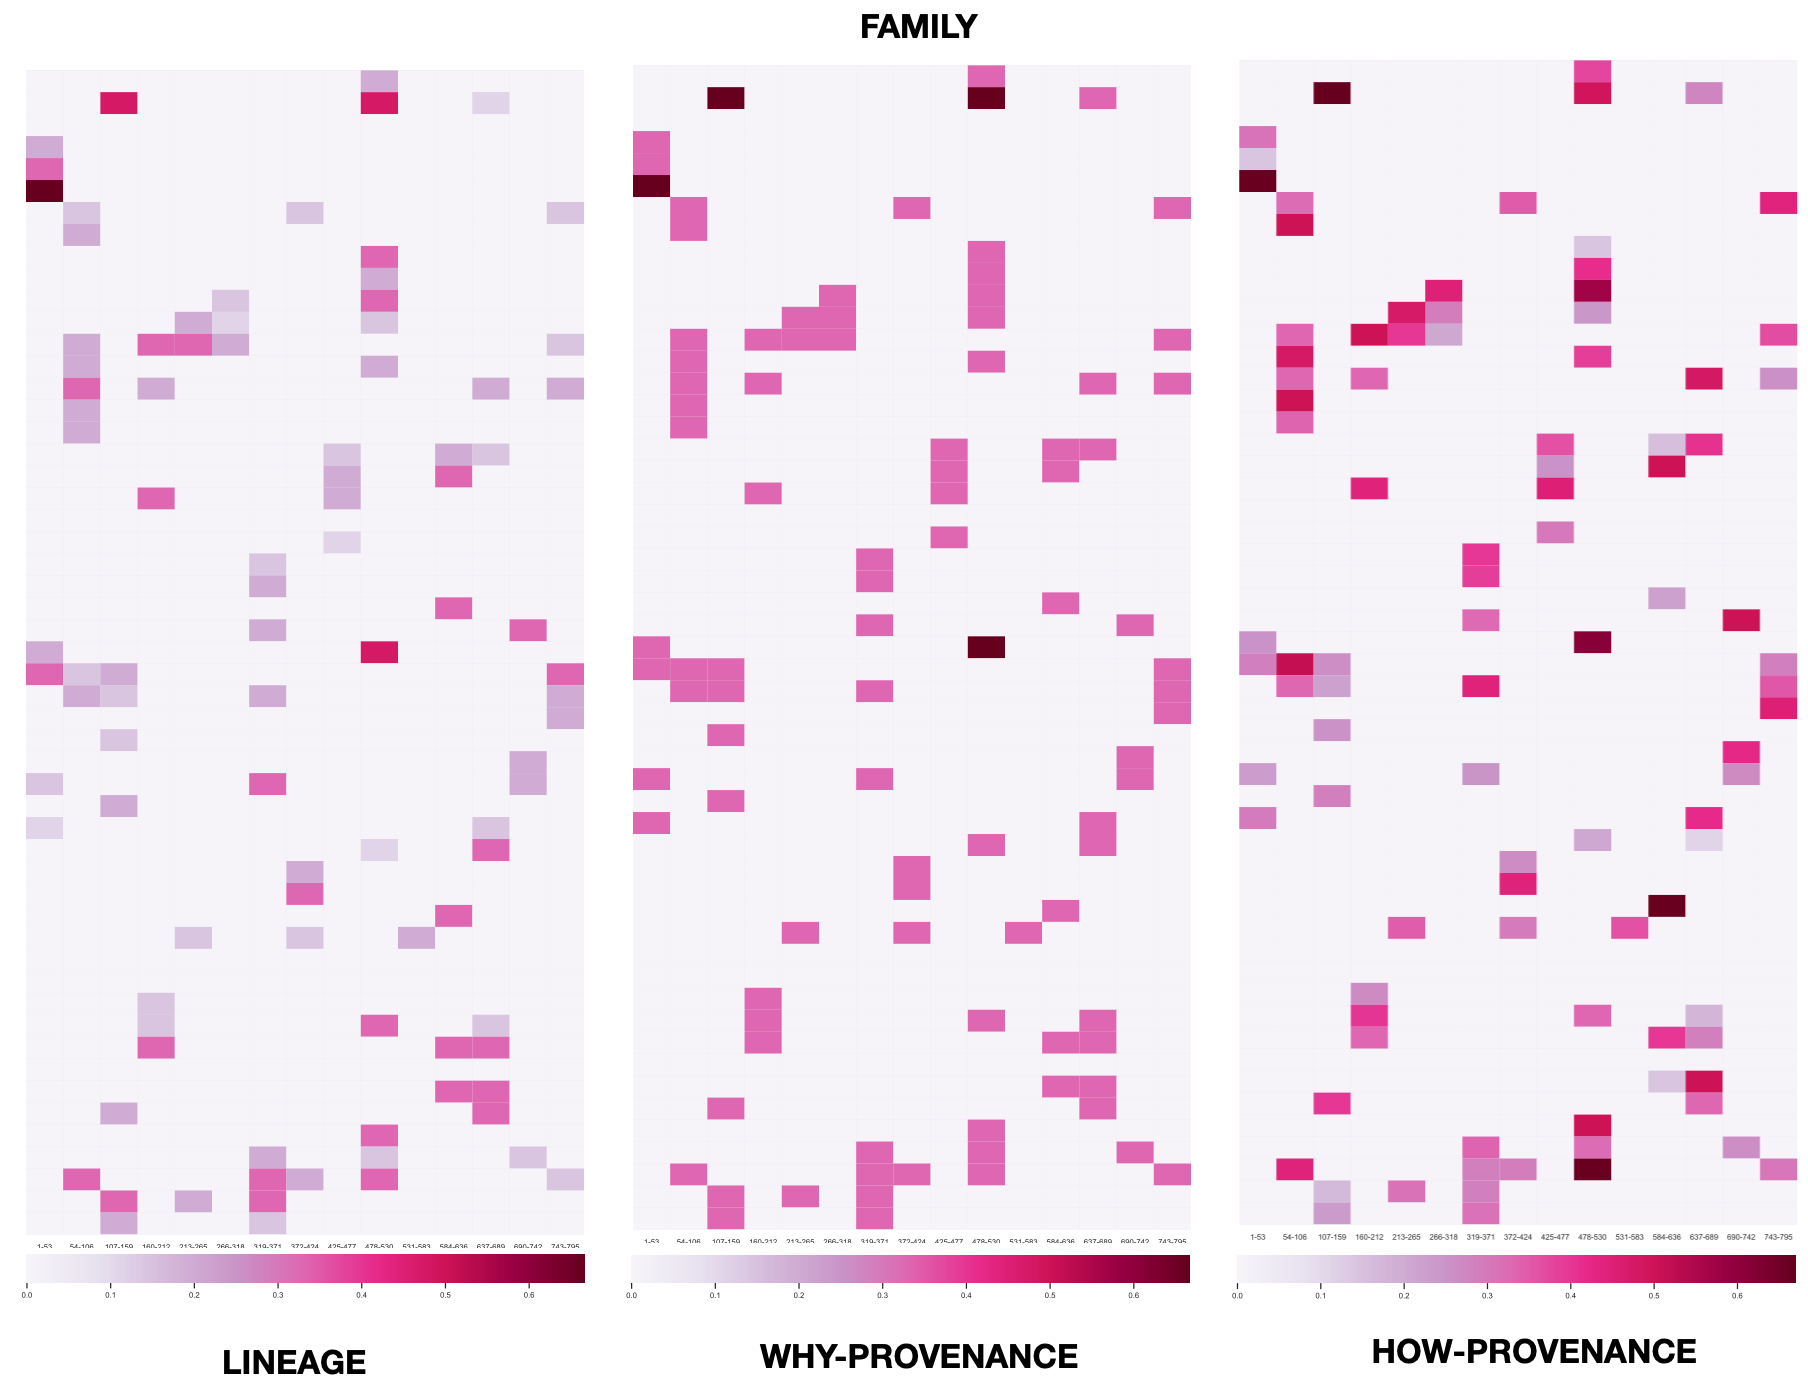
\includegraphics[width=1\textwidth]{figures/synthetic_polynomials_2}
  \caption{Comparison of three DS on the same table \texttt{family} after the distribution computed on provenances randomly generated.}
  \label{figure:comparison_on_synthetic_polynomials_2}
\end{figure}

One may ask now if it is possible to obtain results whose heat maps are visibly different. 
Consider for this Figure \ref{figure:comparison_on_synthetic_polynomials_2}. 
The figure reports a distribution of credit performed on \texttt{family} through the generation of \emph{synthetic} polynomials. 
In this last case, we did not produce full-fledged queries. Rather, we randomly generated provenance polynomials that might be the how-provenance of randomly generated synthetic queries. 
An example of such synthetic polynomial is:
\[
3 f_1^3 c2f_1^2 c_1^2 + 2 f_1 c2f_2^3 c_2^3 + 4 f_5 c2f_{17}^4 c_{18}^3
\] 
As can be seen, we made sure to also include coefficients and exponents that differ from $1$.
Its corresponding why-provenance is: 
\[
\{ \{f_1, c2f_1, c_1\}, \{f_1, c2f_2, cf_2\}, \{ f_5, c2f_{17}, c_{18}\} \}
\] 

its lineage is: 
\[
\{f_1, f_5, c2f_1, c_1, c2f_1, c2f_2, c2f_{17}, c_1, c_2, c_{18} \}
\]
 
These types of polynomials are not impossible to obtain. 
They can be obtained by writing nested queries with join and union operations that use multiple times the same tuples (thus the presence of exponents bigger than $1$) and that use the same combination of operations more than once (thus the presence of coefficients for monomials bigger than $1$). 
We randomly generated a set of $100$ such polynomials. 

Using how-provenance, this is the distribution obtained from the example polynomial we are considering:
\[
f_1 = \frac{59}{315}, f_5 = \frac{1}{18}, c2f_1 = \frac{2}{21}, c2f_2 = \frac{2}{15}, 
c2f_{17}=\frac{2}{9} , c_1 = \frac{2}{21}, c_2 = \frac{2}{15}, c_{17} = \frac{1}{6} 
\]

Using why-provenance, this is the output:
\[
f_1 = \frac{2}{9}, f_5 = \frac{1}{9}, c2f_1 = \frac{1}{9}, c2f_2 = \frac{1}{9}, 
c2f_{17}=\frac{1}{9} , c_1 = \frac{1}{9}, c_2 = \frac{1}{9}, c_{17} = \frac{1}{9} 
\]

Finally, with lineage, this is the distribution:
\[
f_1 = \frac{1}{8}, f_5 = \frac{1}{8}, c2f_1 = \frac{1}{8}, c2f_2 = \frac{1}{8}, 
c2f_{17}=\frac{1}{8} , c_1 = \frac{1}{8}, c_2 = \frac{1}{8}, c_{17} = \frac{1}{8} 
\]

To highlight how the distributions behave differently with these polynomials, consider tuple $f_5$.
$f_5$ receives the highest quantity of credit when we use the lineage-based distribution. Why-provenance and how-provenance reduce its quantity of credit since more information is available for the computation and the algorithms weigh less and less its role. 

Generally speaking, the more complex the distribution, the more polarized the credit is toward the tuples that are used more frequently or with a higher impact in the production of the output tuple. 
Looking at the heat-maps of Figure \ref{figure:comparison_on_synthetic_polynomials_2}, it appears that lineage tends to distribute credit more ``equally'' among the tuples, with only one or two tuples receiving higher quantities of credit, primarily because they are used in many different queries. 

Why-provenance produces more tuples that are rewarded with high values of credit. Moreover, it appears that the other tuples that are not on the top of the spectrum are rewarded even more evenly compared to the DS based on lineage. That is, why-provenance, in this case, rewarded many tuples with roughly the same quantity of credit, and few tuples (but more compared to the DS based on lineage) with higher quantities of credit.
This is due to the fact that why-provenance not only rewards the presence of a tuple in the computation but also the ways in which it is used.

How-provenance, finally, produces the distribution more sensible to the way a tuple is used in a query. Compared to the previous two DS, it also takes into consideration how many times a tuple is used, and weighs this factor in the distribution. It is interesting to see how certain tuples that received the lowest values of credit with lineage are now rewarded with higher values, showing that their fundamental role in certain queries outshines the fact that other tuples were used more frequently in the set of queries.

\begin{figure}[]
\centering
  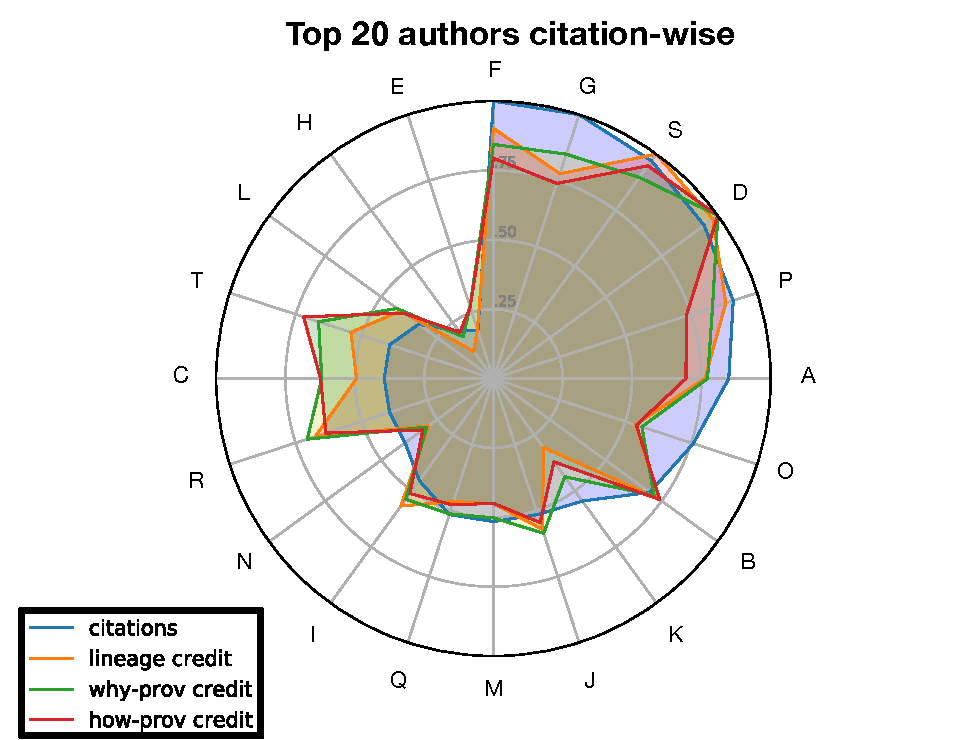
\includegraphics[width=.8\textwidth]{figures/radar_top_synthetic_enhanced}
  \caption{Top 20 authors by number of citations and their credit given through the three different DS.}
  \label{figure:synthetic_authors}
\end{figure}

For our last set of experiments, consider Figure \ref{figure:synthetic_authors}.
We still use the $100$ polynomials described above, and the credit distributed through them. Since these polynomials correspond to queries whose corresponding authors are not easily identifiable, we considered $20$ ``synthetic'' authors and we randomly assigned one author to each tuple in the database. The authors receive ``blocks'' of consecutive tuples, with each block of the size varying between $10$ and $40$. 
Every time a tuple was used in a provenance polynomial, we assigned one citation to the author corresponding to the tuple.  The same author also receives the three different credits assigned to the tuple at the end of the distribution process using the three DS.

Figure \ref{figure:synthetic_authors} presents the radar plot where the 20 authors are sorted based on the normalized number of received citations, together with the corresponding normalized quantities of credits.
Credit presents a different behavior from the one of citations, and each form of credit, i.e. the credit obtained from the different DS, behaves differently from the others.
It appears, for example, that authors T, C, and R that are low in the number of citations, are still rewarded more than other more cited authors in terms of credit.
This is because, even if the tuples of these authors received fewer citations, they still received more credit than other more cited tuples. This shows how credit can be an effective new method to use together with traditional citations to reward curators, highlighting aspects that are lost using the traditional bibliometrics.

The three DS are all effective ways to distribute credit and there is not one distribution that is preferable to the other all the time. It all depends on the needs of the users. 
Lineage is to be preferred when users only want to see the tuples used in queries and to reward more the tuples that are used in many queries. It only rewards based on the \emph{presence} of the tuples. 
Why-provenance is more versatile when users also want to take into consideration how many ways a tuple is used, thus, in a way, its \emph{versatility} inside the queries that used it.
Finally, how-provenance also counts how many times a tuple is used, its \emph{frequency} in the computation of a query. 